\chapter*{Annexe}
\phantomsection
\addcontentsline{toc}{chapter}{Annexe}

\appendix
\section*{Extrais du code SQL des tables}

\noindent CREATE TABLE `parcs` (\\
	`id` bigint(20) UNSIGNED NOT NULL,\\
	`nom\_parc` varchar(255) NOT NULL,\\
	`description` varchar(255) NOT NULL,\\
	`adresse` varchar(255) NOT NULL,\\
	`nombre\_batteries` varchar(255) NOT NULL,\\
	`user\_id` bigint(20) UNSIGNED NOT NULL,\\
	`systeme\_parametre\_id` bigint(20) UNSIGNED NOT NULL,\\
	`created\_at` timestamp NULL DEFAULT NULL,\\
	`updated\_at` timestamp NULL DEFAULT NULL\\
	) ENGINE=InnoDB DEFAULT CHARSET=utf8mb4 COLLATE=utf8mb4\_unicode\_ci;\\

\noindent CREATE TABLE `batteries` (\\
`id` bigint(20) UNSIGNED NOT NULL,\\
`nom` varchar(255) NOT NULL,\\
`capacite\_nominal` varchar(255) NOT NULL,\\
`date\_installation` date NOT NULL,\\
`technologie` varchar(255) NOT NULL,\\
`marque` varchar(255) NOT NULL,\\
`parc\_id` bigint(20) UNSIGNED NOT NULL,\\
`parametre\_batterie\_id` bigint(20) UNSIGNED NOT NULL,\\
`created\_at` timestamp NULL DEFAULT NULL,\\
`updated\_at` timestamp NULL DEFAULT NULL\\
) ENGINE=InnoDB DEFAULT CHARSET=utf8mb4 COLLATE=utf8mb4\_unicode\_ci;\\


\noindent CREATE TABLE `lectures` (\\
`id` bigint(20) UNSIGNED NOT NULL,\\
`tension` decimal(8,2) NOT NULL,\\
`courant` decimal(8,2) NOT NULL,\\
`temperature` decimal(5,2) NOT NULL,\\
`soc` int(11) NOT NULL,\\
`dod` int(11) NOT NULL,\\
`horodatage` timestamp NOT NULL DEFAULT current\_timestamp()\\
 ON UPDATE current\_timestamp(),\\
`batterie\_id` bigint(20) UNSIGNED NOT NULL,\\
`created\_at` timestamp NULL DEFAULT NULL,\\
`updated\_at` timestamp NULL DEFAULT NULL\\
) ENGINE=InnoDB DEFAULT CHARSET=utf8mb4 COLLATE=utf8mb4\_unicode\_ci;\\


\section{Les organigrammes du système}
\subsection{Initialisation et mesure}




\begin{figure}[H]
	\centering
	\begin{subfigure}{0.5\textwidth} % Largeur de la première sous-figure
		\centering
	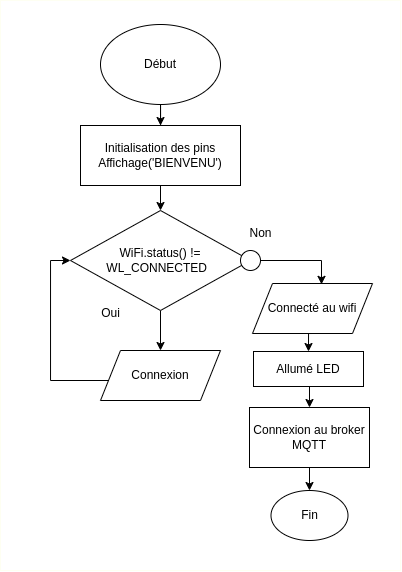
\includegraphics[width=\textwidth]{./img/organigramme/initialisation.png}
	\caption{Organigramme d'initialisation}
	\label{fig:initialisation}
	\end{subfigure}
	\hfill
	\begin{subfigure}{0.45\textwidth} % Largeur de la deuxième sous-figure
		\centering
		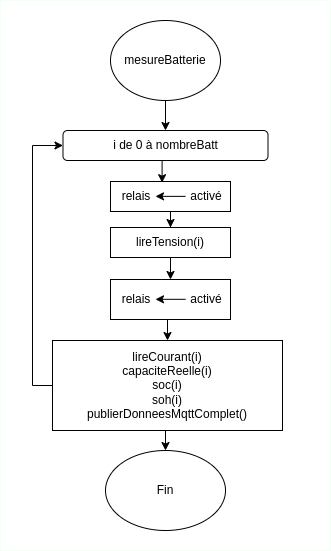
\includegraphics[width=\textwidth]{./img/organigramme/mesure.png}
		\caption{Organigramme de mesure}
		\label{fig:organigramme_mesure}
	\end{subfigure}
	\caption{Organigrammes du processus d'initialisation et de la mesure}
	\label{fig:organigrammes_principal_mesure}
\end{figure}

\subsection{Processus principal et mesure}

\begin{figure}[H]
	\centering
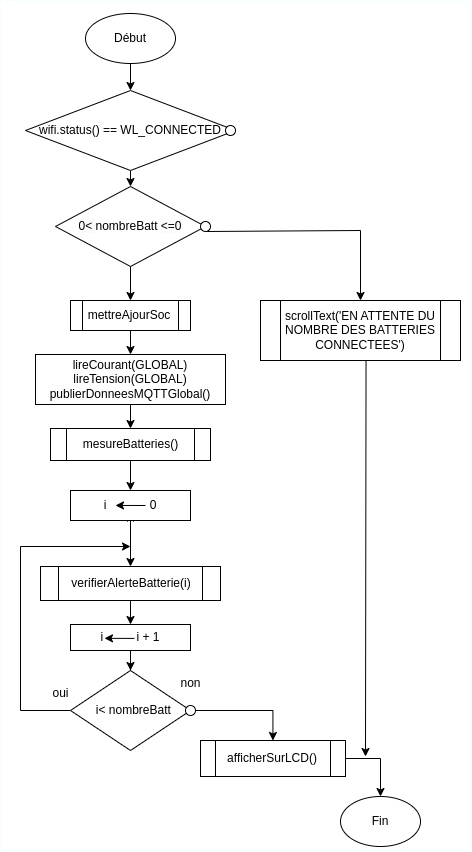
\includegraphics[width=10cm]{./img/organigramme/principale1.png}
\caption{Organigramme principal}
\label{fig:organigramme_principal}
\end{figure}

\section*{Extrait du code source}

\begin{lstlisting}[caption=Code de monitoring des batteries]
// ******************** IMPORTATION *************************** //
#include <LiquidCrystal_I2C.h>
#include <Wire.h>
#include <WiFi.h>
#include <PubSubClient.h>
#include <ArduinoJson.h>
//********** DEFINITION DES PINS POUR LES CAPTEURS *************//
//******************** RELAIS ************************//
#define RELAIS_REGULATEUR 5
#define RELAIS_BATTERIE_1 18
#define RELAIS_BATTERIE_2 19
#define RELAIS_BATTERIE_3 23
//******************** COURANT ************************************//
#define ACS712_BAT1 36
#define ACS712_BAT2 39
#define ACS712_BAT3 25
#define ACS712_GLOBAL 26
//******************** TEMPERATURE ********************************//
#define LM35_BAT1 34
#define LM35_BAT2 35
#define LM35_BAT3 32
//******************** DIVISEUR DE TENSION ************************//
#define DIV_TENSION_BAT1 15
#define DIV_TENSION_BAT2 27
#define DIV_TENSION_BAT3 14
#define DIV_TENSION_GLOBAL 12
//******************** LED ***************************************//
#define LED_PIN 4
//******************** MODULE GSM ********************************//
#define RXD2 16  
#define TXD2 17
#define DDT 1.5
#define NUM_SAMPLES 10
//*********************Initialisation du LCD I2C*******************//
LiquidCrystal_I2C lcd(0x27, 16, 2);
const String phoneNumber = "+261340585428";
const String message = "Bienvenue sur le systeme de monitoring des batteries. Le dispositif est connecte au Wi-Fi et au GSM.";  
const char* ssid = "Airtel_4G_SMARTBOX_2538"; 
const char* password = "C707680D"; 
const char* mqtt_server = "192.168.1.116"; 
const int mqtt_port = 1883;
const char* mqtt_topic_batteries = "batteries";
const char* mqtt_topic_batteriesGlobal = "batteriesGlobal";
const char* mqtt_topic_alerts = "alerts";
const char* mqtt_topic_parametreBatterie = "parametreBatterie";
const int maxBatteries = 3;
float batteries[maxBatteries][12]; 
int nombreBatteries = 0;
WiFiClient espClient;
PubSubClient client(espClient);
const float ACS712_SENSITIVITY = 0.100; 
const float DIVISEUR_TENSION_RATIO = 0.1; 
const float capaciteNominaleBat1 = 100.0;
const float capaciteNominaleBat2 = 100.0;
const float capaciteNominaleBat3 = 100.0;
float courantBat1, courantBat2, courantBat3;
float tensionBat1, tensionBat2, tensionBat3;
float temperatureBat1, temperatureBat2, temperatureBat3;
float socBat1, socBat2, socBat3; 
float sohBat1, sohBat2, sohBat3; 
float capaciteReelleBat1 = 100.0; 
float capaciteReelleBat2 = 100.0;
float capaciteReelleBat3 = 100.0;
float dodBat1, dodBat2, dodBat3; 
unsigned long dernierTempsMesure = 0;
const unsigned long TEMPS_STABILISATION = 2000; 
float courantGlobal, tensionGlobal;
bool gsmReady = false;
int nombreBatteriesConnectees = 0; 
const float referenceVoltage = 3.3; 
const float R1 = 4000.0;  
const float R2 = 1000.0;   
const float ADC_MAX = 4095.0;
const float VREF = 3.3; 
// ================SETUP =========== =====
void setup() {
Serial.begin(115200);
Serial2.begin(9600, SERIAL_8N1, RXD2, TXD2); 
pinMode(RELAIS_REGULATEUR, OUTPUT);
pinMode(RELAIS_BATTERIE_1, OUTPUT);
pinMode(RELAIS_BATTERIE_2, OUTPUT);
pinMode(RELAIS_BATTERIE_3, OUTPUT);
pinMode(LED_PIN, OUTPUT);
digitalWrite(LED_PIN, LOW);  
lcd.init();
lcd.backlight();
lcd.clear();
lcd.setCursor(0, 0);
scrollText("Bienvenue sur Monitoring des Batteries", 0, 300);
socBat1 = 100; 
socBat2 = 100;
socBat3 = 100;
connectToWiFi();
if (WiFi.status() == WL_CONNECTED) {
while (!gsmReady) {
if (checkGSM()) {
digitalWrite(LED_PIN, HIGH);
lcd.clear();
lcd.setCursor(0, 0);
lcd.print("GSM Connecte");
delay(1000);
sendSMS(phoneNumber, message);  
gsmReady = true;  } }}
 else {
digitalWrite(LED_PIN, LOW);
lcd.clear();
lcd.setCursor(0, 0);
lcd.print("WiFi NOK");}
if (WiFi.status() == WL_CONNECTED) {
digitalWrite(LED_PIN, HIGH);
lcd.clear();
lcd.setCursor(0, 0);
lcd.print("WiFi Connecte");
delay(1000);
} else {
digitalWrite(LED_PIN, LOW);
lcd.clear();
lcd.setCursor(0, 0);
lcd.print("WiFi NOK");
}
client.setServer(mqtt_server, mqtt_port);
client.setCallback(callback);
reconnectMQTT();
}
// === LOOP ===
void loop() {
if (WiFi.status() == WL_CONNECTED) {
if (!client.connected()) {
reconnectMQTT();
}
if( 0 < nombreBatteriesConnectees &&  nombreBatteriesConnectees <= 3){
mettreAJourSoC();
// Lire les mesures globales
courantGlobal = lireACS712(26 , 1.65);
tensionGlobal = lireTensionDiviseur(DIV_TENSION_GLOBAL);
publierDonneesMQTTGlobal( tensionGlobal ,courantGlobal );
// Mesurer les tensions, courants et temperatures des batteries
mesurerBatteries();
// Verifier les conditions d'alerte pour chaque batterie
verifierAlerteBatterie(batteries[0][0], socBat1, temperatureBat1, RELAIS_BATTERIE_1 , courantBat1, tensionBat1 , socBat1);
verifierAlerteBatterie(batteries[1][0], socBat2, temperatureBat2, RELAIS_BATTERIE_2 ,  courantBat2, tensionBat2 , socBat2);
verifierAlerteBatterie(batteries[2][0], socBat3, temperatureBat3, RELAIS_BATTERIE_3 ,  courantBat3, tensionBat3 , socBat3);
afficherSurLCD();
}else{scrollTextNonBlocking("EN ATTENTE DU NOMBRE DES BATTERIES CONNECTEES", 0, 300); }
client.loop();}
delay(500);}
unsigned long previousMillis = 0;
int scrollIndex = 0;
bool isScrolling = false;
void scrollTextNonBlocking(String message, int row, int delayTime) {
static String scrollingMessage;
static int messageLength;
static int displayWidth = 16;
if (!isScrolling) {
scrollingMessage = message;
messageLength = message.length();
scrollIndex = 0;
isScrolling = true;}
unsigned long currentMillis = millis();
if (currentMillis - previousMillis >= delayTime) {
previousMillis = currentMillis;
if (scrollIndex <= messageLength - displayWidth) {
lcd.setCursor(0, row);
lcd.print(scrollingMessage.substring(scrollIndex, scrollIndex + displayWidth));
scrollIndex++;
} else {
isScrolling = false;}}}
void scrollText(String message, int row, int delayTime) {
int messageLength = message.length();
int displayWidth = 16; 
if (messageLength <= displayWidth) {
lcd.setCursor(0, row);
lcd.print(message);
delay(delayTime);
} else {
for (int i = 0; i <= messageLength - displayWidth; i++) { 
lcd.setCursor(0, row);
lcd.print(message.substring(i, i + displayWidth)); }}}
void connectToWiFi() {
lcd.setCursor(0, 0);
lcd.print("Connexion WiFi");
WiFi.begin(ssid, password);
while (WiFi.status() != WL_CONNECTED) {
delay(500);
lcd.setCursor(0, 1);
lcd.print("Connexion...");}
lcd.clear();
lcd.setCursor(0, 0);
lcd.print("WiFi Connecte");
lcd.setCursor(0, 1);
lcd.print(WiFi.localIP());
delay(1000);}
void callback(char* topic, byte* payload, unsigned int length) {
String message = "";
for (unsigned int i = 0; i < length; i++) {
message += (char)payload[i];}
DynamicJsonDocument doc(2048); 
DeserializationError error = deserializeJson(doc, message);
nombreBatteries = 0;
JsonArray iArray = doc[0]["i"].as<JsonArray>();
JsonArray cArray = doc[0]["c"].as<JsonArray>();
JsonArray cmaArray = doc[0]["cma"].as<JsonArray>();
JsonArray cmiArray = doc[0]["cmi"].as<JsonArray>();
JsonArray temaArray = doc[0]["tema"].as<JsonArray>();
JsonArray tmaArray = doc[0]["tma"].as<JsonArray>();
JsonArray tmiArray = doc[0]["tmi"].as<JsonArray>();
JsonArray dArray = doc[0]["d"].as<JsonArray>();
JsonArray sArray = doc[0]["s"].as<JsonArray>();
int totalBatteries = iArray.size();
nombreBatteries = totalBatteries > maxBatteries ? maxBatteries : totalBatteries;
for (int index = 0; index < nombreBatteries; index++) {
batteries[index][0] = iArray[index].as<float>();
batteries[index][1] = cArray[index].as<float>();
batteries[index][2] = cmaArray[index].as<float>();
batteries[index][3] = cmiArray[index].as<float>();
batteries[index][4] = temaArray[index].as<float>();
batteries[index][5] = tmaArray[index].as<float>();
batteries[index][6] = tmiArray[index].as<float>();
batteries[index][7] = dArray[index].as<float>();
batteries[index][8] = sArray[index].as<float>();}
nombreBatteriesConnectees = nombreBatteries; }
void reconnectMQTT() {
while (!client.connected()) {
Serial.println("Connexion au broker MQTT...");
if (client.connect("")) {
Serial.println("Connecte au broker MQTT");
if (client.subscribe(mqtt_topic_parametreBatterie)) {
Serial.println("Abonne au topic: nombreBat");
} else {
Serial.println("Echec de l'abonnement au topic: nombreBat");
}} else {delay(2000);}}}
void publierDonneesMQTT(int numeroBatterie, float tension, float courant, float temperature, float soc, float soh) {
String message = "{\"batterie\": " + String(numeroBatterie) +
", \"tension\": " + String(tension) +
", \"courant\": " + String(courant) +
", \"temperature\": " + String(temperature) +
", \"soc\": " + String(soc) +
", \"soh\": " + String(soh) + "}";
}
void publierDonneesMQTTGlobal(float tension, float courant) {
String message = "{\"Global\": true, \"tension\": " + String(tension) + ", \"courant\": " + String(courant) + "}";
}
void publierAlerteMQTT(int numeroBatterie, const String& typeAlerte, float valeur) {
String message = "{\"batterie\": " + String(numeroBatterie) +
", \"type\": \"" + typeAlerte +
"\", \"valeur\": " + String(valeur) + "}";
}
void afficherSurLCD() {
float *tensions[] = {&tensionBat1, &tensionBat2, &tensionBat3};
float *courants[] = {&courantBat1, &courantBat2, &courantBat3};
float *temperatures[] = {&temperatureBat1, &temperatureBat2, &temperatureBat3};
for (int i = 0; i < nombreBatteriesConnectees; i++) {
lcd.clear();
lcd.setCursor(0, 0);
lcd.print("B");
lcd.print(i + 1);
lcd.print(": ");
lcd.print(*tensions[i], 1);
lcd.print("V ");
lcd.setCursor(0, 1);
lcd.print(*courants[i], 1);
lcd.print("A ");
lcd.print(*temperatures[i], 1);
lcd.print("C");
delay(2000);
}
lcd.clear();
lcd.setCursor(0, 0);
lcd.print("Tension T: ");
lcd.print(tensionGlobal, 1);
lcd.print("V ");
lcd.setCursor(0, 1);
lcd.print("Courant T: ");
lcd.print(courantGlobal, 1);
lcd.print("A");
delay(2000);
}
void creerEtEnvoyerAlerte(int numBatterie, String type, float valeur, float seuil, String messageAlerte, int gravite) {
String message = "{\"idbat\": " + String(batteries[numBatterie][0]) +
", \"Valert\": " + String(valeur, 2) +
", \"Vseuil\": " + String(seuil, 2) +
", \"sms\": \"" + messageAlerte + "\"" +
", \"read\": 0" +
", \"type\": \"" + type + "\"" +
", \"contact\": \"" + String(batteries[numBatterie][1]) + "\"" +
", \"gravite\": " + String(gravite) +
"}";
}
void verifierDoD(int numBatterie, float dod, int &gravite , int relaisBatterie) {
if (dod < batteries[numBatterie][7] * 0.5) {
gravite = 4;
creerEtEnvoyerAlerte(numBatterie, "dod", dod, batteries[numBatterie][7],
"Tres bas : infarieur a 50% du seuil.", gravite);
envoyerAlerteEtIsolerBatterie(numBatterie,"Tres bas : inferieur a 50% du seuil.",relaisBatterie,String(batteries[numBatterie][1]));
} else if (dod < batteries[numBatterie][7] * 0.75) {
gravite = max(gravite, 3);
creerEtEnvoyerAlerte(numBatterie, "dod", dod, batteries[numBatterie][7],
"Bas : inferieur a 75% du seuil.", gravite);
} else if (dod < batteries[numBatterie][7]) {
gravite = max(gravite, 2);
creerEtEnvoyerAlerte(numBatterie, "dod", dod, batteries[numBatterie][7],
"Proche du seuil : " + String(dod, 2) + "%.", gravite);
}}
void verifierTemperature(int numBatterie, float temperature, int &gravite , int relaisBatterie) {
if (temperature > batteries[numBatterie][4]) {
gravite = max(gravite, 4);
creerEtEnvoyerAlerte(numBatterie, "temperature", temperature, batteries[numBatterie][4],
"Temperature elevee : " + String(temperature, 2) + "\textdegree C.", gravite);
envoyerAlerteEtIsolerBatterie(numBatterie,"Temperature elevee : " + String(temperature, 2) + "\textdegree C.",relaisBatterie, String(batteries[numBatterie][1]));
} else if (temperature > batteries[numBatterie][4] * 0.8) {
gravite = max(gravite, 3);
creerEtEnvoyerAlerte(numBatterie, "temperature", temperature, batteries[numBatterie][4],
"Temperature proche du seuil : " + String(temperature, 2) + "\textdegree C.", gravite);
}}
void verifierCourant(int numBatterie, float courant, int &gravite , int relaisBatterie) {
if (courant > batteries[numBatterie][2]) {
gravite = max(gravite, 4);
creerEtEnvoyerAlerte(numBatterie, "courant", courant, batteries[numBatterie][2],
"Courant \'elev\'e : " + String(courant, 2) + "A.", gravite);
envoyerAlerteEtIsolerBatterie(numBatterie,"Courant élevé : " + String(courant, 2) + "A.",relaisBatterie ,String(batteries[numBatterie][1]));
} else if (courant > batteries[numBatterie][3] * 0.75) {
gravite = max(gravite, 3);
creerEtEnvoyerAlerte(numBatterie, "courant", courant, batteries[numBatterie][3],
"Courant élevé proche du seuil : " + String(courant, 2) + "A.", gravite);
} else if (courant < batteries[numBatterie][3]) {
gravite = max(gravite, 3);
creerEtEnvoyerAlerte(numBatterie, "courant", courant, batteries[numBatterie][3],
"Courant faible : " + String(courant, 2) + "A.", gravite);
}}
void verifierAlerteBatterie(int numBatterie, float dod, float temperature, int relaisBatterie, float courant, float tension, float soc) {
int gravite = 1; 
verifierDoD(numBatterie, dod, gravite, relaisBatterie);
verifierTemperature(numBatterie, temperature, gravite,relaisBatterie);
verifierCourant(numBatterie, courant, gravite,relaisBatterie);
}
void envoyerAlerteEtIsolerBatterie(int numBatterie, String messageAlerte, int relaisBatterie , String  phone){
digitalWrite(relaisBatterie, LOW);
String message = messageAlerte + ". Action: Batterie " + String(numBatterie) + " isolee.";
sendSMS(phone, message);
lcd.clear();
lcd.setCursor(0, 0);
lcd.print("Alerte B" + String(numBatterie));
lcd.setCursor(0, 1);
lcd.print(messageAlerte);
delay(3000); }
// === Mesure des batteries ===
void mesurerBatteries() {
int relais[] = {RELAIS_BATTERIE_1, RELAIS_BATTERIE_2, RELAIS_BATTERIE_3};
int acs[] = {ACS712_BAT1, ACS712_BAT2, ACS712_BAT3};
int divTension[] = {DIV_TENSION_BAT1, DIV_TENSION_BAT2, DIV_TENSION_BAT3};
int lm35[] = {LM35_BAT1, LM35_BAT2, LM35_BAT3};
float *tension[] = {&tensionBat1, &tensionBat2, &tensionBat3};
float *courant[] = {&courantBat1, &courantBat2, &courantBat3};
float *temperature[] = {&temperatureBat1, &temperatureBat2, &temperatureBat3};
float *capaciteReelle[] = {&capaciteReelleBat1, &capaciteReelleBat2, &capaciteReelleBat3};
float *soh[] = {&sohBat1, &sohBat2, &sohBat3};
float *soc[] = {&socBat1, &socBat2, &socBat3};
const float* capaciteNominale[] = {&capaciteNominaleBat1, &capaciteNominaleBat2, &capaciteNominaleBat3};
float calibration[] = {2.54692, 2.52200, 1.65};
unsigned long tempsActuel = millis();
float deltaTime = (tempsActuel - dernierTempsMesure) / 1000.0; 
float tensionsTemp[nombreBatteriesConnectees];
float courantsTemp[nombreBatteriesConnectees];
float temperaturesTemp[nombreBatteriesConnectees];
float socsTemp[nombreBatteriesConnectees];
float sohsTemp[nombreBatteriesConnectees];
for (int i = 0; i < nombreBatteriesConnectees; i++) {
digitalWrite(relais[i], HIGH);
delay(TEMPS_STABILISATION);
*courant[i] = lireACS712(acs[i], calibration[i]);
*tension[i] = lireTensionDiviseur(divTension[i]);
*temperature[i] = lireLM35(lm35[i]);
*capaciteReelle[i] = *soc[i] * *capaciteNominale[i] / 100.0;
*soc[i] = calculerSoC(*soc[i], *courant[i], *capaciteNominale[i], deltaTime);
*soh[i] = calculerSOH(*capaciteReelle[i], *capaciteNominale[i]);
tensionsTemp[i] = *tension[i];
courantsTemp[i] = *courant[i];
temperaturesTemp[i] = *temperature[i];
socsTemp[i] = *soc[i];
sohsTemp[i] = *soh[i];
digitalWrite(relais[i], LOW);}
publierDonneesMQTTComplet(nombreBatteriesConnectees, tensionsTemp, courantsTemp, temperaturesTemp, socsTemp, sohsTemp);}
void publierDonneesMQTTComplet(int nombreBatteries, float tensions[], float courants[], float temperatures[], float socs[], float sohs[]) {
String message = "[";
for (int i = 0; i < nombreBatteries; i++) {
message += "{";
message += "\"batterie\": " + String(i + 1) +
", \"tension\": " + String(tensions[i], 2) +
", \"courant\": " + String(courants[i], 2) +
", \"temperature\": " + String(temperatures[i], 2) +
", \"soc\": " + String(socs[i], 2) +
", \"soh\": " + String(sohs[i], 2) +
"}";
if (i < nombreBatteries - 1) {
message += ", ";}}
message += "]";}
float lireACS712(int pin , float vcc_mid) {
int sensorValue = 0;
for (int i = 0; i < NUM_SAMPLES; i++) {
sensorValue += analogRead(pin);
delay(10); }
sensorValue /= NUM_SAMPLES;
float voltage = sensorValue * (referenceVoltage / 4095.0); 
float voltage_out = (voltage + 1.1) * DDT; 
float current = (voltage_out - vcc_mid) / ACS712_SENSITIVITY;
return current;}
float lireTensionDiviseur(int pin) {
int totalADCValue = 0;
int rawValue = analogRead(pin);
float voltage = (rawValue / 4095.0) * 3.3;
for (int i = 0; i < NUM_SAMPLES; i++) {
totalADCValue += analogRead(pin);
delay(10); }
int averageADCValue = totalADCValue / NUM_SAMPLES;
float Vout = (averageADCValue * VREF) / ADC_MAX;  
float Vin = Vout * (R1 + R2) / R2; 
return Vin;}
float lireLM35(int pin) {
int rawValue = analogRead(pin);
float voltage = (rawValue / 4095.0) * 3.3;
return voltage * 100.0;}
float calculerSOH(float capaciteReelle, float capaciteNominale) {
return (capaciteReelle / capaciteNominale) * 100.0;}
float calculerSoC(float socActuel, float courant, float capaciteNominale, float deltaTime) {
float chargePerdue = courant * deltaTime; 
float soc = socActuel - (chargePerdue / capaciteNominale) * 100.0;
if (soc > 100) soc = 100; 
return soc;}
void mettreAJourSoC() {
unsigned long tempsActuel = millis();
float deltaTime = (tempsActuel - dernierTempsMesure) / 1000.0; 
socBat1 = calculerSoC(socBat1, courantBat1, capaciteNominaleBat1, deltaTime);
socBat2 = calculerSoC(socBat2, courantBat2, capaciteNominaleBat2, deltaTime);
socBat3 = calculerSoC(socBat3, courantBat3, capaciteNominaleBat3, deltaTime);
dernierTempsMesure = tempsActuel;
dodBat1 = 100.0 - socBat1;
dodBat2 = 100.0 - socBat2;
dodBat3 = 100.0 - socBat3;}
bool checkGSM() {
Serial2.println("AT");  
delay(1000);           
if (Serial2.available()) {
String response = Serial2.readString();  
if (response.indexOf("OK") != -1) {
return true;}}
return false;  }
void sendSMS(String number, String text) {
if (sendATCommand("AT+CMGS=\"" + number + "\"\r", 2000, ">")) {
Serial2.print(text);
delay(100);
Serial2.write((char)26);  
delay(2000);
if (readSerialResponse().indexOf("OK") != -1) {
Serial.println("Message envoye avec succès.");
} else {
Serial.println("Echec de l'envoi du message.");}}}
bool sendATCommand(String command, const int timeout, String expectedResponse) {
Serial2.println(command);
String response = readSerialResponse();
return response.indexOf(expectedResponse) != -1;}
String readSerialResponse() {
String response = "";
unsigned long startTime = millis();
while (millis() - startTime < 2000) {
if (Serial2.available()) {
response += char(Serial2.read());}}
return response;}
\end{lstlisting}

\begin{figure}[H]
	\centering
	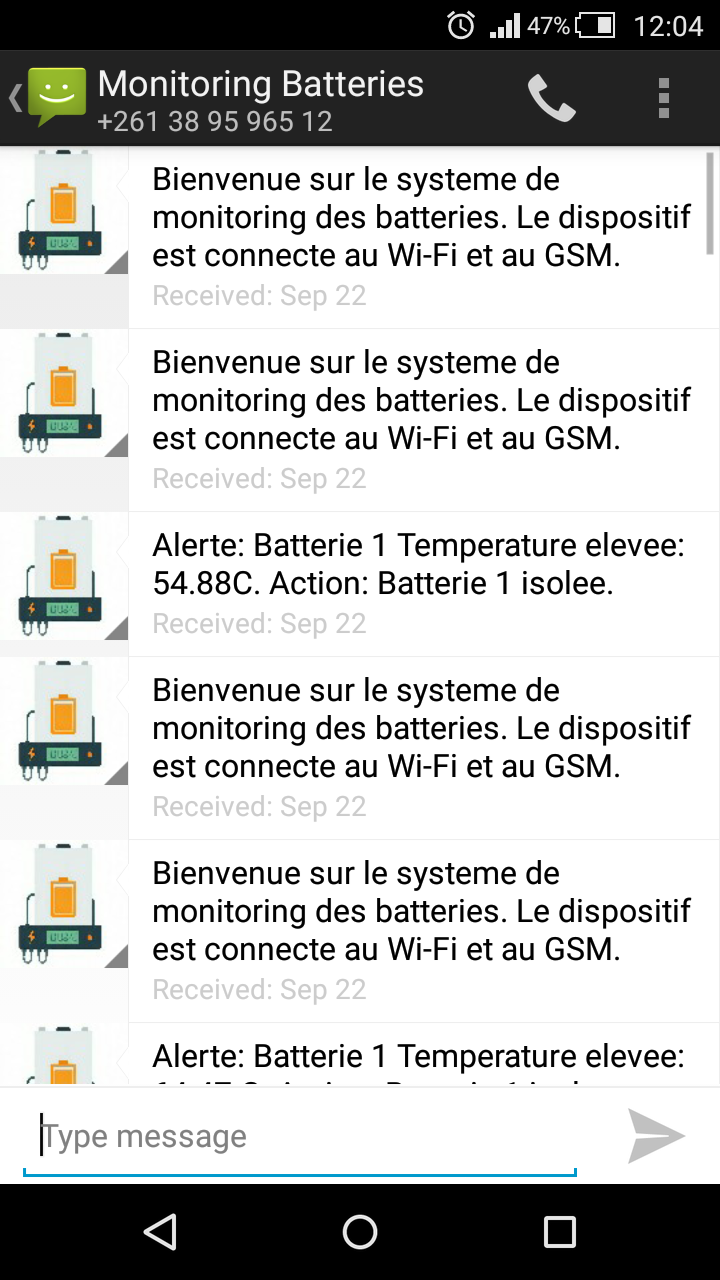
\includegraphics[width=4cm]{./img/composants/sms.png}
	\caption{Les alertes envoyées par SMS provenant du dispositif}
	\label{fig:relais_5vdc}
\end{figure}
